\documentclass[11pt]{article}
\usepackage{amssymb, amsmath, libertine, hyperref, xcolor, booktabs, enumitem, microtype}
\usepackage[T1]{fontenc}
\usepackage[margin=1in]{geometry}
\usepackage{tikz}
\newcommand{\gridxy}[4]{% xmin xmax ymin ymax -- gridlines exactly on the ticks
  \foreach \gX in {#1,...,#2} \draw[gray!25] (\gX,#3) -- (\gX,#4);
  \foreach \gY in {#3,...,#4} \draw[gray!25] (#1,\gY) -- (#2,\gY);}
\definecolor{dark-red}{rgb}{0.4,0.15,0.15}
\hypersetup{colorlinks, linkcolor=dark-red, urlcolor=dark-red}
\setlist[enumerate,1]{label=(\alph*), leftmargin=*, itemsep=5pt, topsep=5pt}
\pagestyle{empty}
\newcommand{\prob}[2]{\medskip\noindent\textbf{\large #1}\hfill\textit{#2}\par\smallskip}

\begin{document}

\begin{center}
{\Large\bfseries Math 111: Calculus \quad Practice Exam 1}\\[4pt]
{For Exam 1, in class on Friday, September 25}
\end{center}

\medskip
\noindent\textbf{What Exam 1 is like.} Four problems in a fifty-minute period, closed-book
and device-free, covering everything through the tangent line approximation
(\S1.1, \S1.3--\S1.8). It is built so that a well-prepared student finishes in about forty
minutes. Each problem is marked holistically on the 0--5 scale: a right answer with no
reasoning is not a 5, and a wrong answer containing a real idea is not a 0. No
differentiation rules are needed anywhere --- everything is done from the definition or
from reasoning about the picture.

\smallskip
\noindent\textbf{How to use this.} Sit down with a blank sheet and forty minutes on a
clock, book closed and phone in another room. Doing that once is worth more than reading
solutions three times. Bring whatever you could not finish to review on Wednesday the 23rd.

\smallskip
\noindent\textbf{One note:} problem 4 uses the tangent line approximation, which we cover
on Monday the 21st. Save it until then.

\bigskip\hrule

\prob{1. The definition, by hand}{about 7 minutes}
Let $f(x) = x^2 - 3x$.
\begin{enumerate}
\item Use the limit definition to compute $f'(2)$. Show the algebra, and do not skip the
step where the $h$ cancels.
\item Use the definition again to find $f'(a)$ for an arbitrary $a$, and check that it
agrees with part (a).
\item In one sentence, say what $f'(2)$ tells you about the graph of $f$ at $x=2$.
\end{enumerate}

\prob{2. Everything from one picture}{about 11 minutes}
The graph of a function $f$ on $[0,7]$ is shown. No formula is given.
\smallskip
\begin{center}
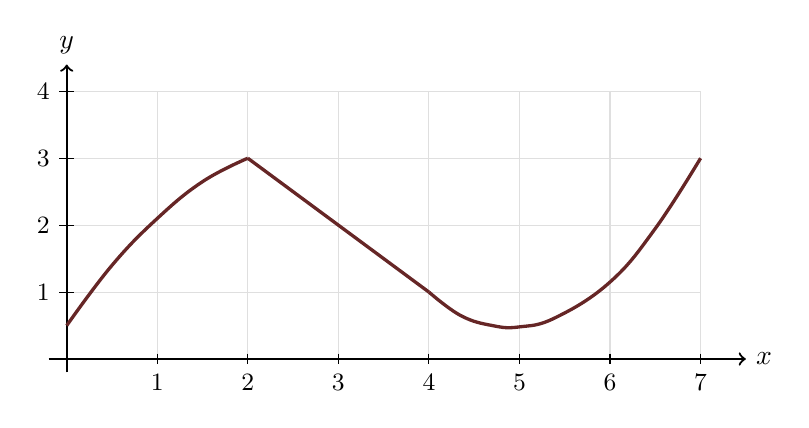
\begin{tikzpicture}[x=1.15cm,y=0.85cm]
  \gridxy{0}{7}{0}{4}
  \draw[->,thick] (-0.2,0) -- (7.5,0) node[right] {$x$};
  \draw[->,thick] (0,-0.2) -- (0,4.4) node[above] {$y$};
  \foreach \x in {1,...,7} \draw (\x,0.08) -- (\x,-0.08) node[below,font=\small] {\x};
  \foreach \y in {1,...,4} \draw (0.08,\y) -- (-0.08,\y) node[left,font=\small] {\y};
  \draw[very thick, dark-red, smooth, tension=0.7]
    plot coordinates {(0,0.5) (0.5,1.4) (1,2.1) (1.5,2.65) (2,3)};
  \draw[very thick, dark-red] (2,3) -- (4,1);
  \draw[very thick, dark-red, smooth, tension=0.7]
    plot coordinates {(4,1) (4.35,0.65) (4.7,0.5) (5,0.48) (5.4,0.62) (6,1.15) (6.5,1.95) (7,3.0)};
\end{tikzpicture}
\end{center}
\begin{enumerate}
\item Sketch $f'$ on $[0,7]$ on axes of your own, marking clearly any place where $f'$
does not exist.
\item At which $x$ in $(0,7)$ does $f'$ fail to exist? Say precisely what goes wrong, and
say whether $f$ is continuous there.
\item On which subintervals of $[0,7]$ is $f'$ increasing? Justify from the graph of $f$
itself, not from your sketch in part (a).
\item Put $f'(1)$, $f'(3)$, and $f'(5)$ in increasing order, and justify from the picture.
\end{enumerate}

\newpage
\prob{3. A reservoir, and what the numbers are worth}{about 11 minutes}
Let $V(t)$ be the volume of water in a reservoir, in millions of gallons, $t$ days after
September 1.
\smallskip
\begin{center}
\begin{tabular}{@{}lrrrrr@{}}
\toprule
$t$ (days) & 0 & 3 & 6 & 9 & 12\\
$V(t)$ (millions of gallons) & 4.0 & 4.9 & 5.5 & 5.8 & 5.9\\
\bottomrule
\end{tabular}
\end{center}
\smallskip
\begin{enumerate}
\item Estimate $V'(6)$. State the units, and write one sentence saying what your estimate
means to somebody who manages the reservoir.
\item Give an estimate of $V'(6)$ that is certainly too large and one that is certainly
too small. Say which is which, and what you are assuming about $V'$ in order to be sure.
\item Is $V'$ increasing or decreasing over these twelve days? What does your answer say
about the reservoir?
\end{enumerate}

\prob{4. The tangent line as an approximation}{about 11 minutes}
\noindent\textit{This problem uses \S1.8, which we cover on Monday, September 21.}
\smallskip

Suppose $f$ satisfies $f(4) = 12$ and $f'(4) = -0.8$, and $f$ is concave down everywhere
near $x=4$.
\begin{enumerate}
\item Write down the tangent line to $f$ at $x=4$ and use it to estimate $f(4.5)$.
\item Is your estimate too large or too small? Justify using the concavity, and draw a
picture that makes the argument visible.
\item Would you use the same method to estimate $f(9)$? Explain what does and does not go
wrong, and say what you would need to know to trust such an estimate.
\end{enumerate}

\end{document}
